\section{Introduction}
\subsection{Shughni}
\par The Shughni language (ISO: sgh; glottolog: shug1248) is a low-resource language. It belongs to the Iranian branch of the Indo-European family \parencite[12]{plungian_study_2022}, and it is spoken by circa 80 000--100 000 people \parencite{edelman_dodykhudoeva_shughni_2009} in two regions: Mountainous Badakhshan Autonomous Region (Tajikistan) and Badakhshan Province (Afghanistan). Both regions have a subregion, where Shughni language is the most spoken native language, the subregions are called 'Shughnon' in Tajikistan and 'Shughnan' in Afghanistan \parencite[2]{parker_shughni_2023}, see Figure \ref{fig:map1} for details. Shughni has a mixed morphological typology type \parencite[94]{parker_shughni_2023}, which means that grammatical meanings can be carried by morphemes, words or clitics. There are three scripts for Shughni language: Latin, Cyrillic and Arabic. The Arabic script is used on the territory of Badakhshan Province of Afghanistan, and Cyrillic and Latin scripts are used in the Mountainous Badakhshan Autonomous Region of Tajikistan. The Latin script was created and gained popularity in 1930s, after it was set as the primary script for teaching in schools on the Shughni-speaking territory of Tajikistan. Later in 1980s a Cyrillic script was created \parencite[788]{edelman_dodykhudoeva_shughni_2009}.
\begin{figure}[h]
    \centering
    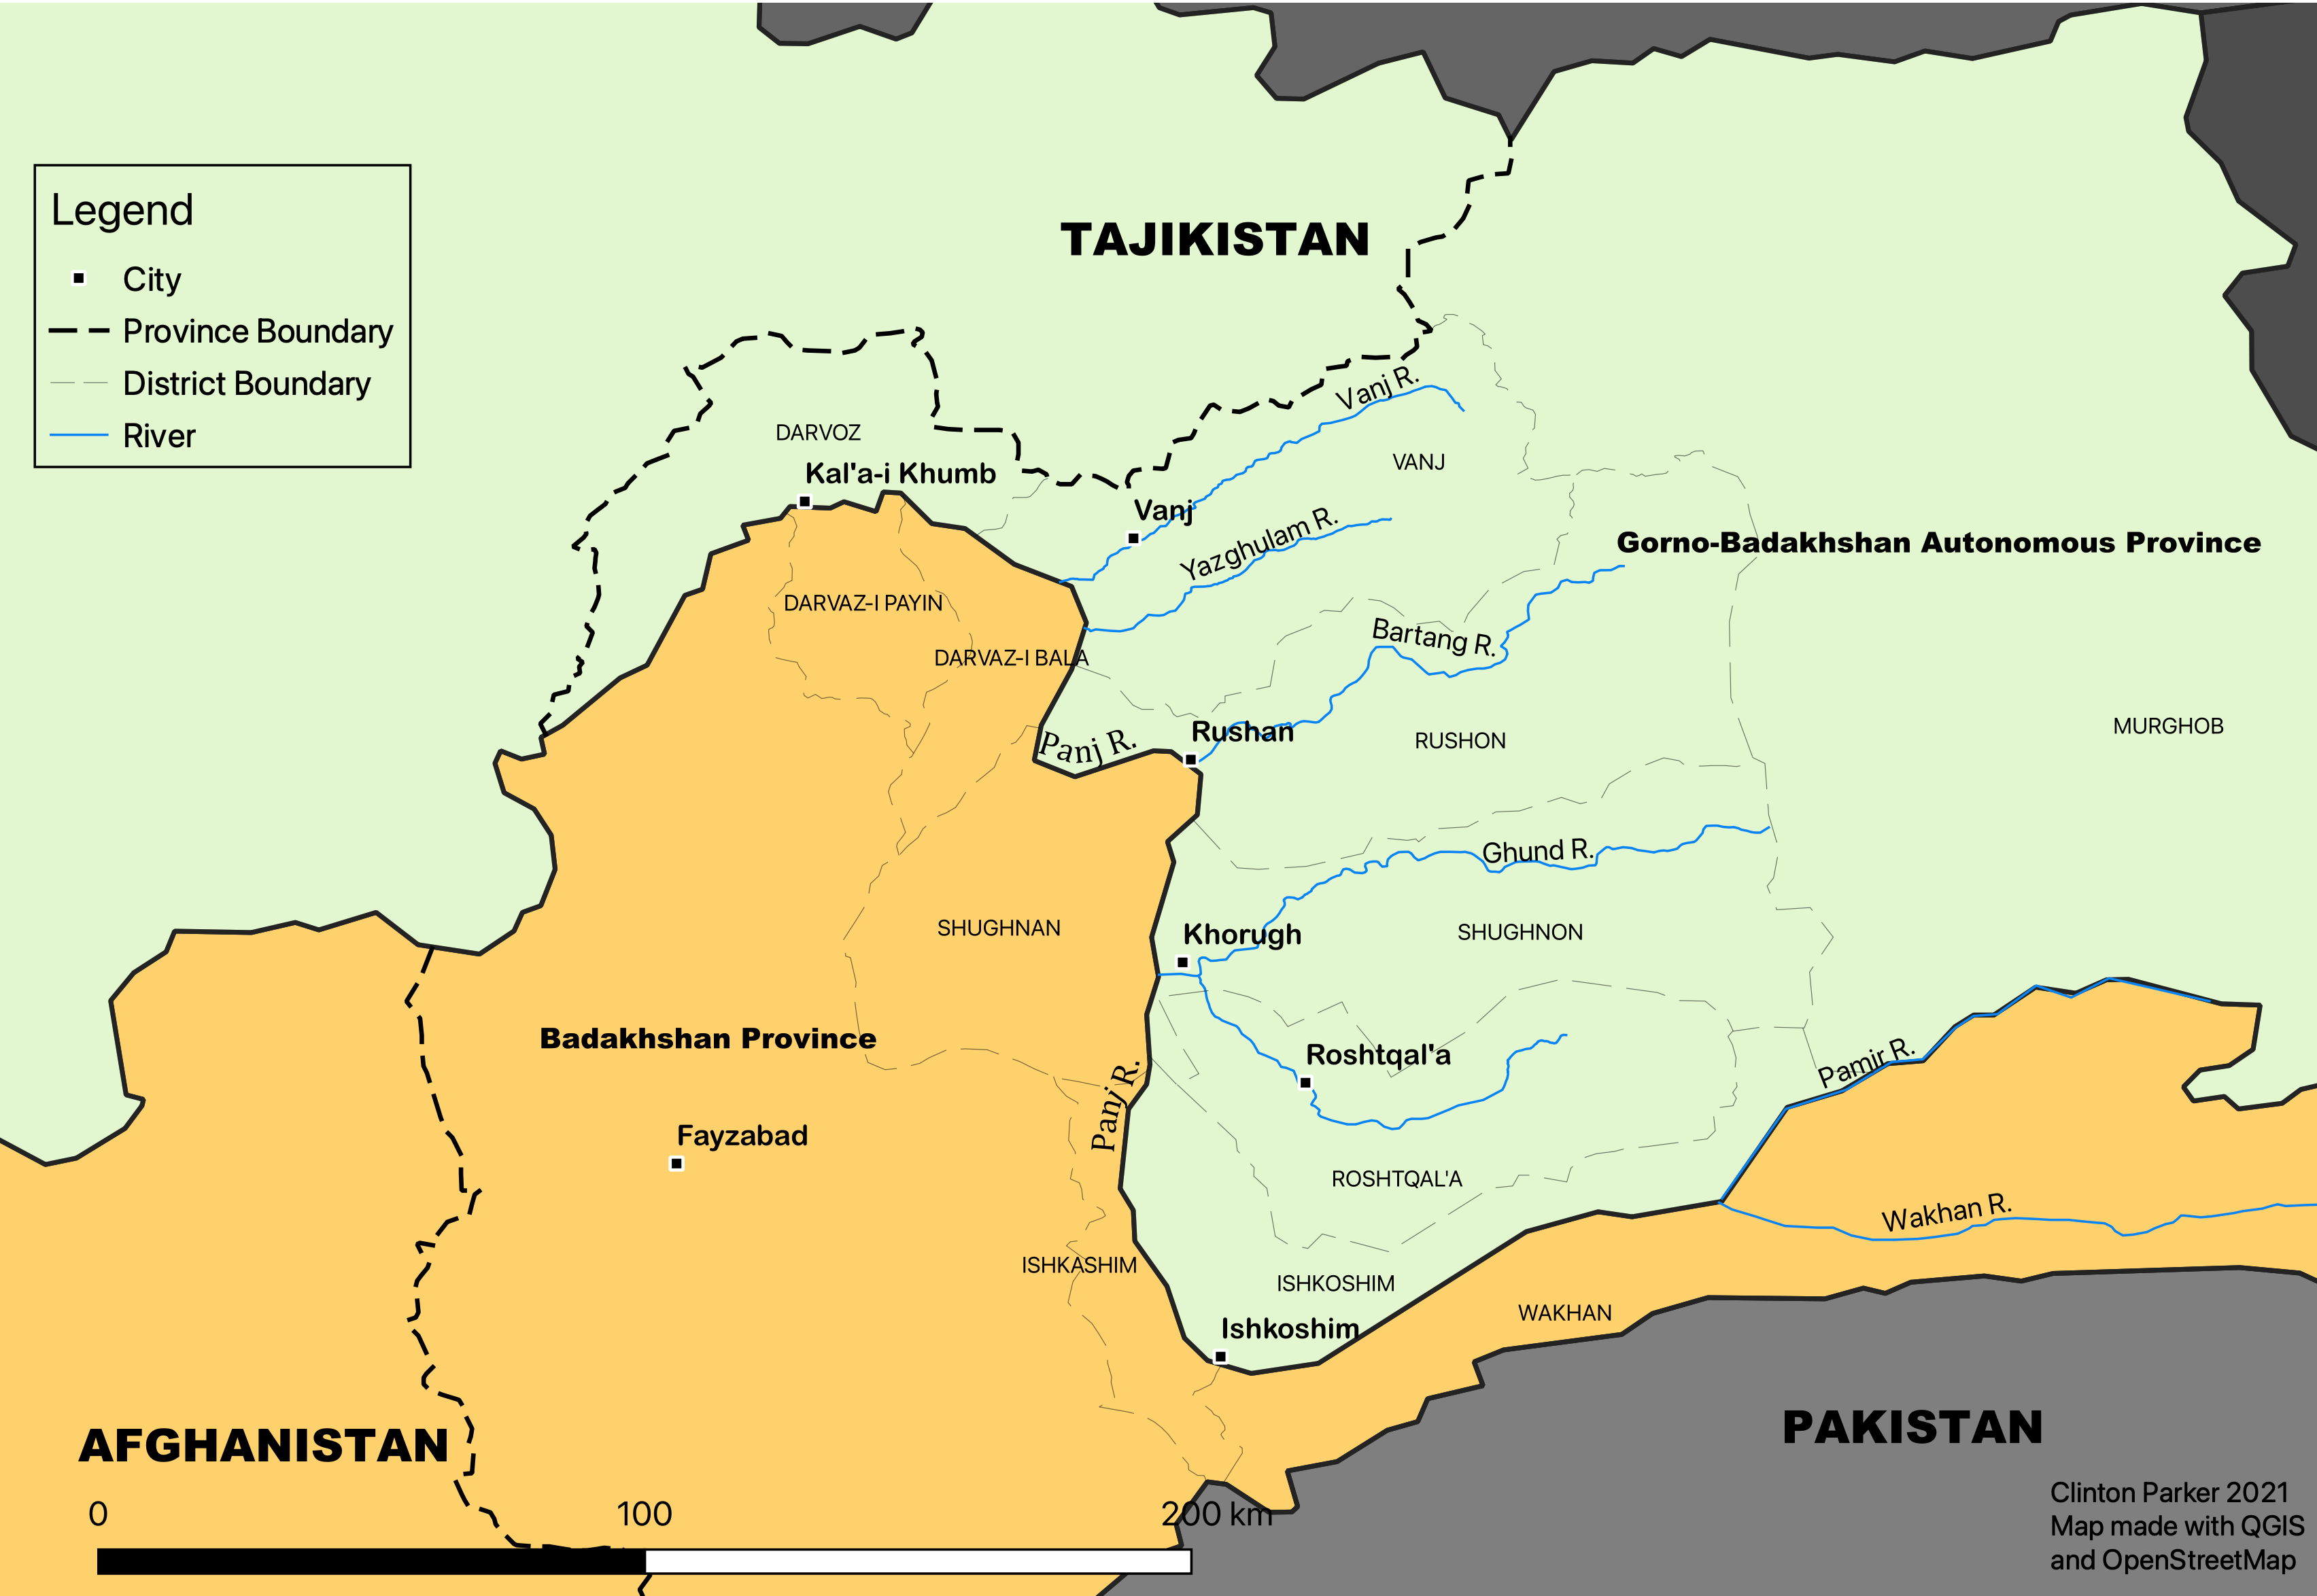
\includegraphics[scale=0.125]{\rootdir/img/map.png}
    \caption{Mountainous Badakhshan Autonomous Province of Tajikistan and Badakhshan Province of Afghanistan, \parencite[Fig 1.1]{parker_shughni_2023}}
    \label{fig:map1}
\end{figure}
\par Morphology analysis tools in question will focus on the variation of Shughni that is spoken in Tajikistan. Cyrillic and Latin script will be supported: the core analysis tool will be implemented in Cyrillic script, and Latin script support will be implemented via transliteration.
\todo{Вы упомянули, что грамматические значения выражаются морфемами и клитиками, имеет смысл упомянуть орфографические конвенции во всех трех (ну или хотя бы двух письменностях), так как если клитики пишутся слитно это важно для работы, если раздельно, то это для работы облегчение, а если то так, то сяк --- значит теоретически интересный случай.}

\subsection{Morphology parsing}
\par Morphological parser is a fundamental tool, a wide range of computational linguistics' tasks \todo{such as ...} rely on some form of morphological model. For morphologically rich languages it is close to impossible to list and manually define all the possible word-forms. The only reasonable way to approach such problem is to model a language's morphology. \todo{Citation needed}
\par For high-resource languages morphology modeling today is usually approached using deep learning (DL) models, which are trained on large amounts of data. \todo{Citation needed} This method is not always available for low-resource languages that lack digital textual data, for such languages linguists apply rule-based approach. \todo{Citation needed} Shughni is a low-resource language with very few data available, which leaves us the rule-based option.
\par The morphological parser will be developed using Helsinki Finite-State Technology (HFST) \parencite{linden_hfst_2009}, which is a tool set for working with rule-based morphology models in a form of transducers. Finite-state transducer (FST) is a finite-state machine that works with two tapes \todo{Стоит как-то отметить, что эти ленточки --- математические абстракции.}: reads strings of text from the input tape and writes strings of text to the output tape. When FST receives an input string, it walks along its characters from one state to another as long as there is a valid transition from the current state with an upcoming letter, see Figure \ref{fig:fst1} for visualization. \todo{Добавьте про конечное состояние: а) что оно маркируется двойным кружочком; б) что их может быть несколько, например, закончить можно было и на work.}
\begin{figure}[!ht]
    \centering
    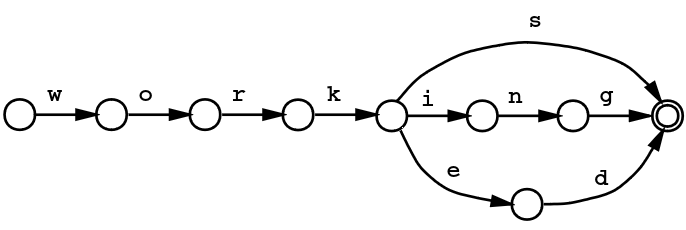
\includegraphics[scale=0.5]{\rootdir/img/transducer1.png}
    \caption{An example of FST for a language where only three words exist: \textit{works}, \textit{working} and \textit{worked}. The word \textit{worker}, for example will not be recognized as a valid word by this FST, since there is no 'd' transition at state \textit{worke}. The only way from \textit{worke} state is via 'd' transition, which corresponds to the \textit{worked} word. \parencite{beesley_fst_2002}}
    \label{fig:fst1}
\end{figure}
\par As FST walks through states (on Fig.\ref{fig:fst1} states are graph's nodes) on each transition (on Fig.\ref{fig:fst1} transitions are graph's edges) it can read an input tape and/or write to the output tape. A syntax for transitions is \textit{'x:y'}, which means "read \textit{x} from input, write \textit{y} to output". Transition will happen only if input matches. With this in mind we can turn FST from Figure \ref{fig:fst1} into a morphological analyser by modifying some transitions (See Fig. \ref{fig:fst1_1}). Syntax \textit{'x:'} means that FST must write nothing to the output tape while still making a transition to the next state if input matches.
\begin{figure}[!ht]
    \centering
    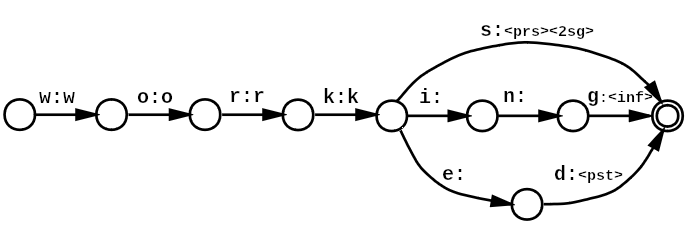
\includegraphics[scale=0.5]{\rootdir/img/transducer1_1.png}
    \caption{A modified version of Figure \ref{fig:fst1} which takes as input \textit{works}, \textit{working}, \textit{worked} and outputs \textit{work<prs><2sg>}, \textit{work<inf>}, \textit{work<pst>} respectively.}
    \label{fig:fst1_1}
\end{figure}

\todo{Если честно, я бы описание работы FST отправил в methods, а здесь бы добавил хоть каких-то интересностей про сам шугнанский. Почему вообще интересно это для условной FST-теории.}